\documentclass[11pt, aspectratio=169, xcolor={dvipsnames}]{beamer}
\usetheme{Madrid}
\usepackage[T1]{fontenc}
\usepackage{lmodern}
\usepackage{booktabs}
\usepackage{array}
\usepackage{tikz}
\usetikzlibrary{positioning,arrows.meta}
\hypersetup{pdfpagemode=UseNone, hidelinks, pdfdisplaydoctitle=true,%
pdftitle={False Alarms from Kernel Tests on Time Series with Long Memory}, pdfauthor={}}
\graphicspath{{figures/}}

% ---- Look ----
\definecolor{ktblue}{HTML}{1F4E8C}
\definecolor{ktred}{HTML}{B3261E}
\setbeamercolor{structure}{fg=ktblue}
\setbeamercolor{palette primary}{bg=ktblue, fg=white}
\setbeamercolor{palette secondary}{bg=ktblue!85!black, fg=white}
\setbeamercolor{palette tertiary}{bg=ktblue!70!black, fg=white}
\setbeamercolor{frametitle}{bg=ktblue, fg=white}
\setbeamercolor{title}{bg=ktblue, fg=white}
\setbeamercolor{block title}{bg=ktblue!15, fg=ktblue!80!black}
\setbeamercolor{block body}{bg=ktblue!5}
\setbeamertemplate{blocks}[rounded][shadow=false]
\setbeamertemplate{navigation symbols}{}
\setbeamerfont{frametitle}{size=\large,series=\bfseries}
\setbeamerfont{block title}{size=\small,series=\bfseries}
\setbeamertemplate{footline}{%
  \leavevmode\hbox{%
  \begin{beamercolorbox}[wd=.8\paperwidth,ht=2.4ex,dp=1ex,left,leftskip=3mm]{palette primary}%
    \usebeamerfont{footline}\insertsectionhead\end{beamercolorbox}%
  \begin{beamercolorbox}[wd=.2\paperwidth,ht=2.4ex,dp=1ex,right,rightskip=3mm]{palette primary}%
    \usebeamerfont{footline}\insertframenumber{} / \inserttotalframenumber\end{beamercolorbox}}}

% ---- Helpers ----
\newcommand{\fig}[2][0.5]{\begin{center}\includegraphics[height=#1\textheight]{#2}\end{center}\vspace{-3mm}}
% why{evidence type}: the reasoning behind the claim in the slide title.
\newenvironment{why}[1]{\begin{block}{Why\hfill\normalfont\footnotesize Evidence: #1}\small
  \setlength{\leftmargini}{1.2em}}{\end{block}}
% thread: one line that links this slide to the next step of the argument.
\newcommand{\thread}[1]{\par\vspace{-1mm}{\footnotesize\itshape\color{ktblue}\hfill$\rightarrow$ #1\par}}

\title[False alarms on long-memory data]{False Alarms from Kernel Tests\\on Time Series with Long Memory}
\subtitle{Where the tests fail, why they fail, and what to do about it}
\author{}
\date{Call with Gareth Peters, Wednesday 4 November 2026}

\begin{document}
\section{The problem}
\begin{frame}[plain]\titlepage\end{frame}

\begin{frame}
\frametitle{Research problem and questions (1)}
\begin{block}{Setting}\small
We observe one path $(X_t,Y_t)_{t\le n}$ and test $H_0$: the processes $X$ and $Y$ are independent. Each process may have long memory, $\rho(k)\sim ck^{2H-2}$ with $H\in(1/2,1)$. Our baseline is fractional Gaussian noise (fGn). The statistic is $T_n=nV_n$, the Gaussian-kernel HSIC $V$-statistic with median bandwidth. For split MMD, $H_0$ is that the two halves of one stationary series share a distribution. A rule estimates the critical value $\hat c_{n,1-\alpha}$ from the same path. The rule is calibrated if $\Pr_{H_0}(T_n>\hat c_{n,1-\alpha})\to\alpha$.
\end{block}
\begin{block}{Research questions}\small
\begin{enumerate}
\item \textbf{Scope of theory.} Do the published assumptions exclude these processes?
\item \textbf{Calibration.} For which statistic, critical-value rule, $H$ and $n$ does the size depart from $\alpha=5\%$?
\item \textbf{Attribution.} Does the departure come from memory, from other process features (heavy tails, nonlinear dynamics, seasonality), or from their interaction?
\item \textbf{Procedure.} Which procedure keeps size and power, and what limits it?
\end{enumerate}
\end{block}
\end{frame}

\begin{frame}
\frametitle{Research problem and questions (2): the intuition in plain English}
\begin{block}{What goes wrong}\small
\begin{itemize}
\setlength{\itemsep}{0pt}
\item A test must learn how large its statistic gets when nothing is going on. It learns this threshold from the data it is testing.
\item That works if distant stretches of a series are nearly unrelated, because one path then holds many separate pieces of evidence.
\item Under long memory, distant stretches stay related, so one path holds far fewer pieces than $n$ suggests. Two unrelated series can wander in step for long periods by chance.
\item A rule that learns from short stretches can miss these slow swings. Its threshold can then be too low, and the test reports links that do not exist.
\item Seasonal patterns add a second route. Two unrelated seasonal series keep one timing gap for the whole path, so more data repeats that gap and does not average it out.
\end{itemize}
\end{block}
\begin{block}{What we want to find out}\small
Did the theory already rule these data out? How wrong are the tests, and under which rules? Is memory to blame, or something else? What should someone do in practice?
\end{block}
\end{frame}

\begin{frame}
\frametitle{Why calibration is in doubt: where the validity argument breaks}
\begin{center}
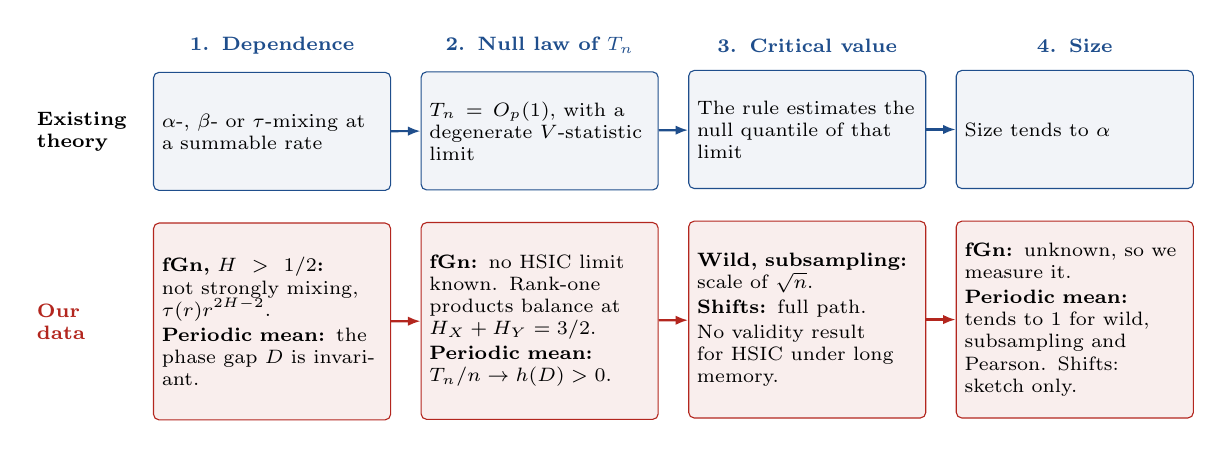
\begin{tikzpicture}[every node/.style={font=\scriptsize, align=left},
  ok/.style={draw=ktblue, fill=ktblue!6, rounded corners=2pt, inner sep=3pt, text width=28mm, minimum height=15mm},
  bad/.style={draw=ktred, fill=ktred!8, rounded corners=2pt, inner sep=3pt, text width=28mm, minimum height=25mm},
  hd/.style={font=\scriptsize\bfseries, text=ktblue, text width=28mm, align=center},
  lab/.style={font=\scriptsize\bfseries, text width=12mm, align=left},
  arr/.style={-{Latex[length=1.6mm]}, ktblue, thick},
  brk/.style={-{Latex[length=1.6mm]}, ktred, thick}]
\node[hd] (h1) at (0,0) {1. Dependence};
\node[hd, right=3.5mm of h1] (h2) {2. Null law of $T_n$};
\node[hd, right=3.5mm of h2] (h3) {3. Critical value};
\node[hd, right=3.5mm of h3] (h4) {4. Size};
\node[ok, below=1mm of h1] (a1) {$\alpha$-, $\beta$- or $\tau$-mixing at a summable rate};
\node[ok, below=1mm of h2] (a2) {$T_n=O_p(1)$, with a degenerate $V$-statistic limit};
\node[ok, below=1mm of h3] (a3) {The rule estimates the null quantile of that limit};
\node[ok, below=1mm of h4] (a4) {Size tends to $\alpha$};
\node[bad, below=4mm of a1] (b1) {\textbf{fGn, $H>1/2$:} not strongly mixing, $\tau(r)\gtrsim r^{2H-2}$.\\[1pt]\textbf{Periodic mean:} the phase gap $D$ is invariant.};
\node[bad, below=4mm of a2] (b2) {\textbf{fGn:} no HSIC limit known. Rank-one products balance at $H_X+H_Y=3/2$.\\[1pt]\textbf{Periodic mean:} $T_n/n\to h(D)>0$.};
\node[bad, below=4mm of a3] (b3) {\textbf{Wild, subsampling:} scale of $\sqrt n$.\\[1pt]\textbf{Shifts:} full path.\\[1pt]No validity result for HSIC under long memory.};
\node[bad, below=4mm of a4] (b4) {\textbf{fGn:} unknown, so we measure it.\\[1pt]\textbf{Periodic mean:} tends to 1 for wild, subsampling and Pearson. Shifts: sketch only.};
\node[lab, left=1.5mm of a1] {Existing theory};
\node[lab, left=1.5mm of b1, text=ktred] {Our data};
\foreach \x/\y in {a1/a2,a2/a3,a3/a4}{\draw[arr] (\x) -- (\y);}
\foreach \x/\y in {b1/b2,b2/b3,b3/b4}{\draw[brk] (\x) -- (\y);}
\end{tikzpicture}
\end{center}
\vspace{-2mm}
\begin{why}{source audit and Proposition 1}
The guarantee needs all four links. Our data break the first link, so links 2 to 4 lose their support. Without a null limit we cannot derive the size for fGn.
\end{why}
\thread{So the size must be measured. First, the objects we compare.}
\end{frame}

\section{What we compare}
\begin{frame}
\frametitle{Three kinds of statistic, each needing a critical value}
\small
\renewcommand{\arraystretch}{1.25}
\begin{tabular}{@{}>{\bfseries}p{0.3\linewidth}p{0.2\linewidth}p{0.44\linewidth}@{}}
\toprule
Statistic & Input & Null hypothesis \\
\midrule
Split MMD & One series & The two halves have the same distribution \\
HSIC, distance covariance & Two aligned series & The two processes are independent \\
Pearson correlation & Two aligned series & No linear link. This is the linear reference. \\
\bottomrule
\end{tabular}
\vspace{2mm}
\begin{block}{The critical-value rule is the part that uses the dependence}\small
A rule must estimate the null quantile of the statistic from one dependent path. We therefore treat the rule as a factor in its own right, alongside the statistic.
\end{block}
\begin{why}{logic of the design}
We run several rules on the same statistic. An oracle that size-adjusts the bare statistic then shows what each rule costs.
\end{why}
\thread{The rules differ in how much of the path they use, which matters if memory is slow.}
\end{frame}

\begin{frame}
\frametitle{Long memory: non-summable autocovariance reduces the information in a path}
\fig[0.5]{memory_paths}
\begin{why}{exact calculation (Proposition 2)}
The gap between two half-sample means has variance $(4-2^{2H})\,m^{2H-2}$. At $H=0.5$ this shrinks like $1/m$. At $H=0.8$ it shrinks only like $m^{-0.4}$. The paths are single simulated draws.
\end{why}
\end{frame}

\begin{frame}
\frametitle{Three critical-value rules: what each one uses from the path}
\fig[0.42]{yardsticks}
\begin{why}{explanation, consistent with the measured rates}
\begin{itemize}
\item Subsampling uses windows of $\sqrt n$ points, which is 44 points at $n=2000$. The wild rule weights lags on the same scale.
\item Long memory moves slowly, so a short stretch can miss most of the movement, and the critical value can come out too low.
\end{itemize}
\end{why}
\thread{This suggests a rule that uses the full path.}
\end{frame}

\begin{frame}
\frametitle{The circular shift breaks the cross-dependence and keeps each series' memory}
\fig[0.42]{shift_diagram}
\begin{why}{construction (Chwialkowski and Gretton, 2014)}
\begin{itemize}
\item The order inside $Y$ barely changes, so $Y$ keeps its own memory. Only the alignment with $X$ moves.
\item Repeating this over many offsets gives the critical value from the full series. We exclude offsets below $0.1n$.
\item Their result assumes mixing, and fGn with $H>1/2$ is not mixing.
\end{itemize}
\end{why}
\thread{Next: how we test these rules, and why this design.}
\end{frame}

\section{How we test it, and why}
\begin{frame}
\frametitle{How we test each question, and why this design}
\footnotesize
\renewcommand{\arraystretch}{1.2}
\begin{tabular}{@{}>{\bfseries}p{0.15\linewidth}>{\raggedright}p{0.38\linewidth}>{\raggedright\arraybackslash}p{0.41\linewidth}@{}}
\toprule
Question & How we test it & Why this design \\
\midrule
1. Theory & Read the stated conditions in the primary sources. Check fGn against each one. & A warning by implication appears only in the conditions, so we check them directly. \\
2. Calibration & Monte Carlo under a known null. Cross rule, $H$ and $n$. Compare Hermite ranks one and two. & No HSIC null limit is available, so we measure size. The rank calculation predicts where the scale changes. \\
3. Attribution & Factorial design: one process feature at a time, crossed with $H$. Holm correction. & It separates a feature's effect alone from its interaction with memory. \\
4. Procedure & Power at matched size. Seasonal adjustment, then rerun the rules. & A test can hold size by having no power. Raw power is not comparable across oversized rules. \\
Mechanism & Prove exact results where the structure allows. & Simulation gives size at design points. A proof gives the limit and the reason. \\
External & Stock trade durations as a placebo. & This checks the account on real data. The null is unverified, so the rates are descriptive. \\
\bottomrule
\end{tabular}
\end{frame}

\begin{frame}
\frametitle{Monte Carlo design: the null is true by construction}
\begin{center}
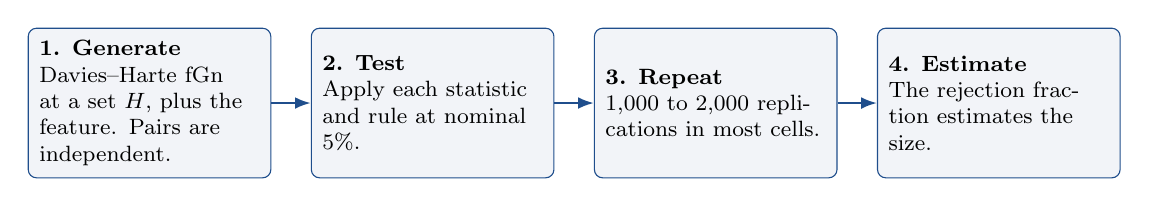
\begin{tikzpicture}[node distance=5mm, every node/.style={font=\footnotesize, align=left},
  box/.style={draw=ktblue, fill=ktblue!6, rounded corners=3pt, inner sep=4pt, text width=28mm, minimum height=19mm},
  arrow/.style={-{Latex[length=2mm]}, ktblue, thick}]
\node[box] (a) {\textbf{1. Generate}\\Davies--Harte fGn at a set $H$, plus the feature. Pairs are independent.};
\node[box, right=of a] (b) {\textbf{2. Test}\\Apply each statistic and rule at nominal 5\%.};
\node[box, right=of b] (c) {\textbf{3. Repeat}\\1,000 to 2,000 replications in most cells.};
\node[box, right=of c] (d) {\textbf{4. Estimate}\\The rejection fraction estimates the size.};
\draw[arrow] (a) -- (b);
\draw[arrow] (b) -- (c);
\draw[arrow] (c) -- (d);
\end{tikzpicture}
\end{center}
\vspace{-1mm}
\begin{why}{design of the study}
\begin{itemize}
\item \textbf{Known null.} We set the generator, so a rejection cannot reflect a real effect.
\item \textbf{Shared baseline.} All generators share one code path, so the Gaussian row is a direct baseline.
\item \textbf{Stated uncertainty.} With 1,000 replications, a 5\% rate has a 95\% Wilson interval of about $\pm1.4$ points. This covers counting error only.
\item \textbf{Fixed in advance.} For EXP2, a design record set the hypotheses and generator checks before the main run.
\end{itemize}
\end{why}
\end{frame}

\begin{frame}
\frametitle{The experiments: what each one varies and what it answers}
\footnotesize
\renewcommand{\arraystretch}{1.1}
\begin{tabular}{@{}>{\bfseries}p{0.075\linewidth}>{\raggedright}p{0.23\linewidth}>{\raggedright}p{0.44\linewidth}>{\raggedright\arraybackslash}p{0.17\linewidth}@{}}
\toprule
Name & Question & What we vary & Size per cell \\
\midrule
EXP1 & Q2: calibration & $H$ from 0.5 to 0.9. Ten pairs with $H_X+H_Y$ from 1.3 to 1.7. MMD on rank-one and rank-two features. & $n\le4000$, 1,000--2,000 runs \\
EXP2 & Q3: attribution & Seven generators (Gaussian, heavy-tailed, nonlinear, seasonal) crossed with $H=0.5, 0.7, 0.8$. & $n=500, 2000$, 1,000 runs \\
EXP3 & Q4: power & Power with each rule tuned to a true 5\%. Linear, squared and seasonal-scale links. MMD mean shift. & $n=500, 2000$, 1,000 runs each way \\
EXP4 & Q4: adjustment & Remove the mean, then the scale, then use an estimated period. Slow scale drift. & $n=500, 2000$, 1,000 runs \\
EXP5, EXP6 & Q2, Q4: robustness & Larger $n$, and a shift scaled to the null spread. Bandwidth at 0.5, 1, 2, 4 times the median. & $n\le8000$, 144--1,000 runs \\
Stocks & External check & AAPL, MSFT, NVDA trade durations, January to June 2024, windows at least 20 sessions apart. & $n\le2000$, 500 pairs \\
\bottomrule
\end{tabular}
\end{frame}

\section{Q1: scope of theory}
\begin{frame}
\frametitle{Q1: the published conditions exclude fGn with $H>1/2$, mostly by implication}
\footnotesize
\renewcommand{\arraystretch}{1.05}
\begin{tabular}{@{}>{\raggedright}p{0.3\linewidth}>{\raggedright}p{0.3\linewidth}>{\raggedright\arraybackslash}p{0.34\linewidth}@{}}
\toprule
\textbf{Source} & \textbf{Stated condition} & \textbf{fGn with $H>1/2$} \\
\midrule
Gretton et al.\ (HSIC, MMD), Sz\'ekely et al.\ (dCov) & i.i.d. & Excluded \\
Chwialkowski, Gretton 2014 (shift HSIC) & $\beta$-mixing at a polynomial rate & Excluded: not strongly mixing \\
Chwialkowski et al.\ 2014 (wild) & $\sum_r r^2\tau(r)^{1/2}<\infty$ & Excluded: our derivation gives $\tau(r)\gtrsim r^{2H-2}$ \\
Ghoshal, Shao 2026 (self-normalized) & Summable strong mixing & Excluded \\
Diz-Castro et al.\ 2026 (HSIC wild) & Near-epoch dependence on a $\beta$-mixing process & Excluded for $H_X+H_Y\ge3/2$. Open below \\
Betken, Dehling, arXiv 2107.03041 (dCov) & Covers Gaussian-subordinated long memory & Covered in part. No Gaussian-kernel HSIC limit \\
\bottomrule
\end{tabular}
\begin{why}{audit of primary sources}
The conditions rule these data out but give no size for the failure, so we measure it. None of the audited sources treats seasonality.
\end{why}
\end{frame}

\section{Q2: calibration}
\begin{frame}
\frametitle{Q2: with the same generator and $n$, the rule changes the size}
\fig[0.52]{rule_lines}
\begin{why}{measured, 2,000 replications per point}
Only the statistic and rule differ between lines, so they account for the gaps. Part of the excess is not memory: the wild rule already sits at 6.5\% at $H=0.5$.
\end{why}
\thread{Why do distortions start where they do?}
\end{frame}

\begin{frame}
\frametitle{Q2: higher Hermite rank delays the size distortion in split MMD}
\fig[0.42]{mmd_ranks}
\begin{why}{measured, with a classical rank calculation for the shape}
\begin{itemize}
\item Rank $m$ gives a leading covariance of order $\rho(k)^m$. Rank two balances at $H=3/4$. Independent rank-one products balance at $H_X+H_Y=3/2$.
\item The calculation explains the shape. It gives no critical value, and the plots do not locate a proved boundary.
\end{itemize}
\end{why}
\thread{Memory distorts size. Is memory the main cause?}
\end{frame}

\section{Q3: attribution}
\begin{frame}
\frametitle{Q3: in our settings, seasonality distorts size more than memory}
\fig[0.5]{feature_heatmap}
\begin{why}{measured, 1,000 replications per cell, Holm-corrected}
We switch on one feature at a time and cross it with memory. HSIC shift stays between 3.8\% and 7.0\%. The threshold AR adds short-range persistence, so its excess is not purely a nonlinearity effect. The seasonal settings are illustrative and not calibrated to market data.
\end{why}
\thread{The two seasonal forms fail for different reasons.}
\end{frame}

\begin{frame}
\frametitle{Q3: with no memory, a seasonal scale distorts kernel tests unless they use shifts}
\begin{center}
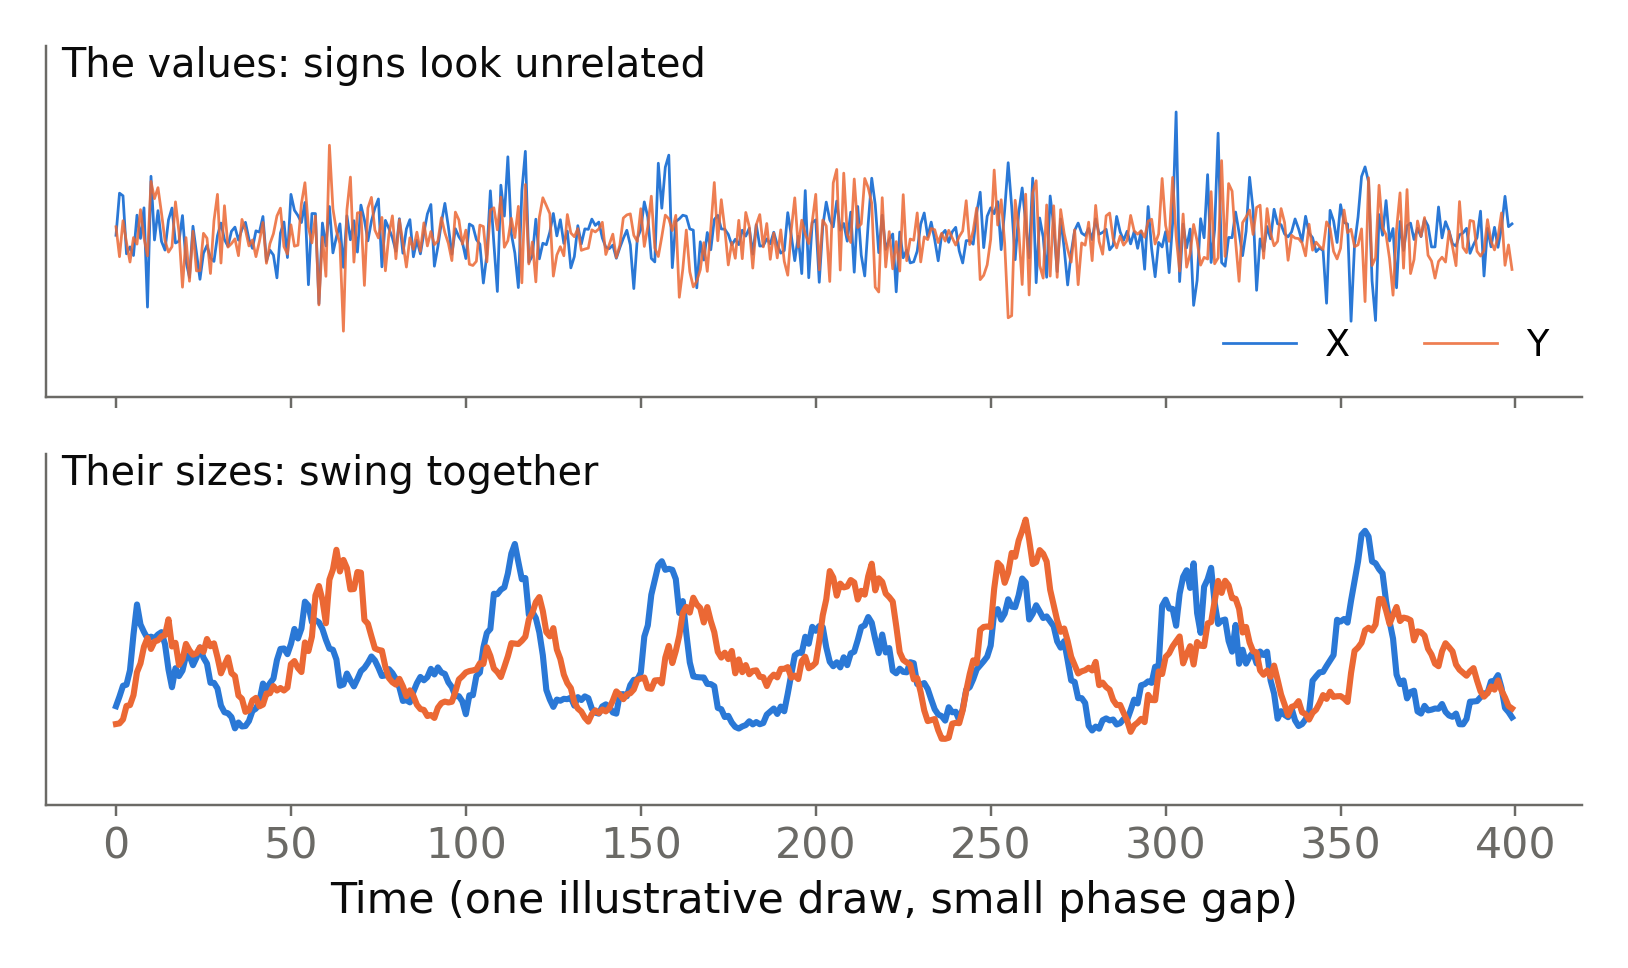
\includegraphics[height=0.42\textheight]{seasonal_scale}\hspace{3mm}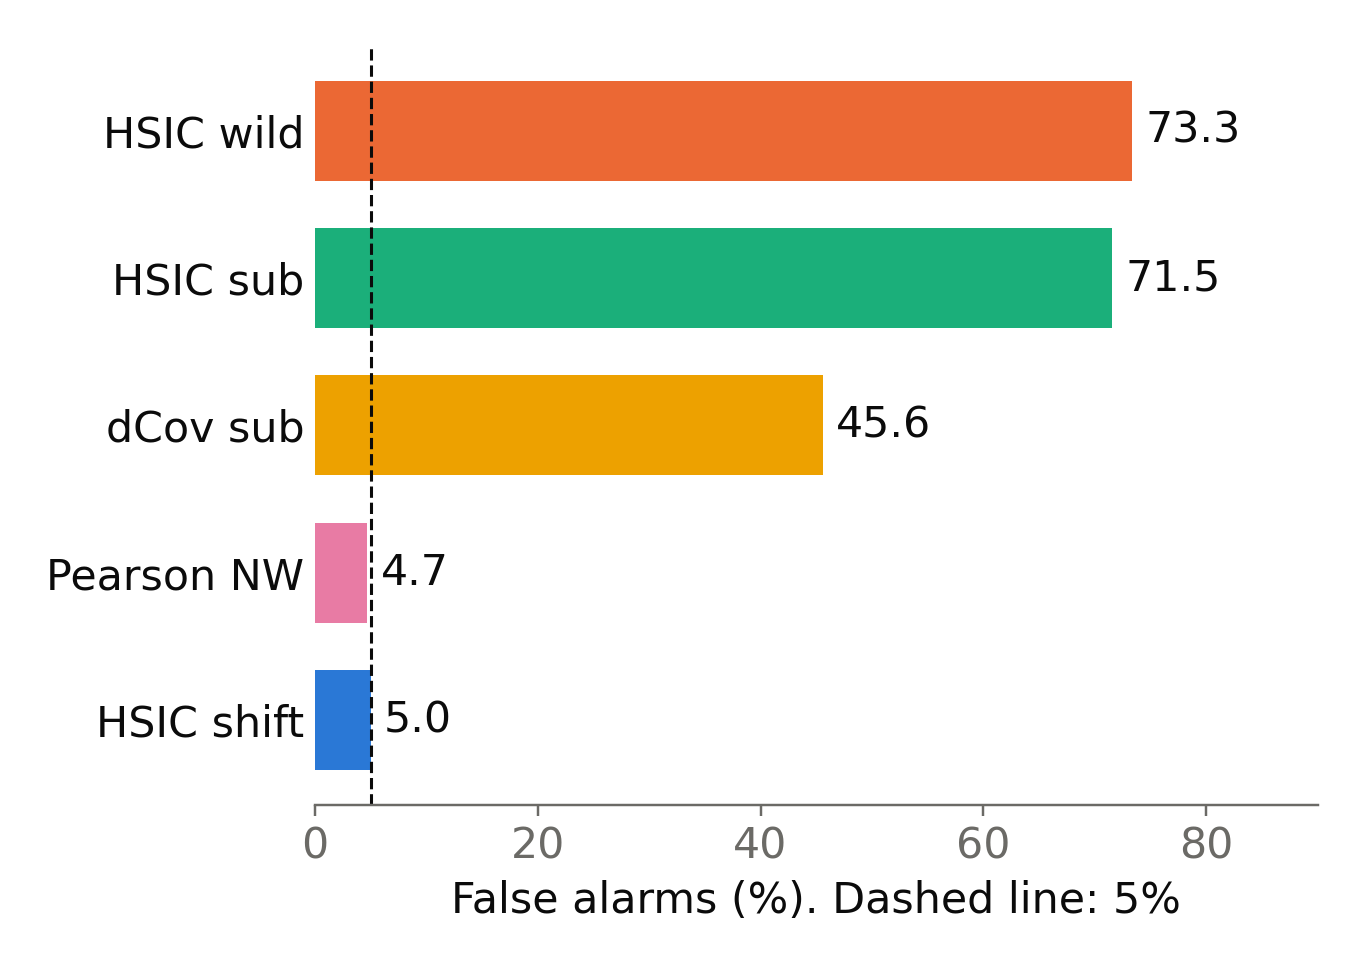
\includegraphics[height=0.42\textheight]{seasonal_bars}
\end{center}
\vspace{-3mm}
\begin{why}{measured, with no proof yet}
These series are independent, and each has its own random phase. HSIC wild, HSIC subsampling and dCov subsampling respond to sizes and reject 46--73\%. HSIC shift rejects 5.0\%. Pearson sees only the linear link and rejects 4.7\%.
\end{why}
\end{frame}

\begin{frame}
\frametitle{Q3: a seasonal mean distorts every independence rule tested except shifts}
\fig[0.42]{phase_gap}
\begin{why}{proved for these rules (Proposition 1), measured for shifts}
\begin{itemize}
\item One path contains one phase gap. The sample correlation converges to a random limit set by that gap.
\item With $P=50$, 46 of 50 gaps give a limit clearly away from zero, which predicts 92\%. Pearson rejects 91.4\%.
\item Shifts re-randomize the gap and stay at 5.8\%. We can only sketch why.
\end{itemize}
\end{why}
\thread{Shifts hold size throughout. Do they do so at the cost of power?}
\end{frame}

\section{Q4: procedure}
\begin{frame}
\frametitle{Q4: shifts keep their power when every rule is tuned to a true 5\%}
\fig[0.42]{power}
\begin{why}{measured at matched size}
\begin{itemize}
\item Shifts stay within 4.9 points of the best other HSIC rule in all 18 cells.
\item Raw power can mislead. HSIC subsampling shows 86.4\% at its nominal critical value and 14.6\% at a true 5\%.
\item The tuning uses the known null, so it checks the rules and is not a method for real data.
\end{itemize}
\end{why}
\thread{Under a shared fixed seasonal phase, shifts still reject 28--34\%, so we adjust first.}
\end{frame}

\begin{frame}
\frametitle{Q4: adjust first, removing the seasonal scale as well as the mean}
\fig[0.42]{adjustment}
\begin{why}{measured, 1,000 replications per cell}
\begin{itemize}
\item Kernel tests respond to the scale, so removing the mean alone barely changes this cell.
\item A period estimated from the data worked as well as the true period.
\item Adjustment costs size under memory. On Gaussian pairs at $H=0.8$, HSIC shift goes from 5.3\% to 6.8\%.
\end{itemize}
\end{why}
\thread{For split MMD, the obstacle is different: information, not calibration.}
\end{frame}

\begin{frame}
\frametitle{Q4: memory caps power against a mean shift for location-invariant tests}
\fig[0.42]{half_mean}
\begin{why}{proved (Proposition 2), measured for MMD}
\begin{itemize}
\item At $n=2000$, a shift of 0.1 is 2.24 null standard deviations at $H=0.5$ and only 0.40 at $H=0.8$.
\item No location-invariant 5\% test can pass 12\% power at $H=0.8$. MMD reaches 6.4--7.5\%.
\item The loss is in the data. It is not a failure of a kernel rule.
\end{itemize}
\end{why}
\thread{The two propositions in full, and what remains unproved.}
\end{frame}

\begin{frame}
\frametitle{Formal results: what we prove and what we do not}
\footnotesize
\begin{columns}[T]
\begin{column}{0.5\textwidth}
\begin{block}{Proposition 1: seasonal mean, any $H\in(0,1)$}\footnotesize
$X_t=\xi_t+a\sin\{2\pi(t+U)/P\}$, and $Y_t$ likewise with an independent phase $V$. Let $D=(U-V)\bmod P$.
\begin{itemize}
\item $r_n\to c(D)=\dfrac{(a^2/2)\cos(2\pi D/P)}{1+a^2/2}$ almost surely.
\item If the critical value is of smaller order than the seasonal term, the size tends to 1 at $P=50$. This covers Pearson NW and EWC, and HSIC wild and subsampling.
\end{itemize}
\textbf{Reason:} one path fixes one gap, so the limit is random and non-zero.
\end{block}
\end{column}
\begin{column}{0.5\textwidth}
\begin{block}{Proposition 2: half-sample mean shift}\footnotesize
$Z_t=\mu+\xi_t+\delta\,\mathbf 1\{t>m\}$, with $n=2m$.
\begin{itemize}
\item $\operatorname{Var}(\Delta_m)=(4-2^{2H})\,m^{2H-2}$, exactly for every $m$.
\item A level-$\alpha$ location-invariant test has power at most $1-\Phi(z_{1-\alpha}-\delta I_n^{1/2})$. Here $I_n$ is the inverse GLS variance of $\hat\delta$.
\item At $n=2000$, $\delta=0.1$: caps of 72\%, 18\%, 12\% at $H=0.5, 0.7, 0.8$.
\end{itemize}
\textbf{Reason:} the bound comes from the information in the data, so it holds for every such test.
\end{block}
\end{column}
\end{columns}
\vspace{-1.5mm}
\begin{alertblock}{Not proved}\scriptsize
The finite-sample size of shifts, which we only simulate. An argument shows the shift rule's size is right asymptotically (inc1, and raw below 3/2), but it rests on an unreviewed preprint. Proved directly: inc1's statistic stays bounded at every $H<1$ at a fixed width. The seasonal-mean sketch lacks uniform convergence and ties. The RKHS Hermite expansion. The seasonal-scale failure, which we only measure.
\end{alertblock}
\end{frame}

\begin{frame}
\frametitle{Q4: what is and is not proved}
\fig[0.33]{limits}
\begin{why}{measured, with wide intervals at large $n$}
\begin{itemize}
\item Shift rates at $H=0.8$ are 5.7\%, 6.3\% and 8.3\% at $n=2000, 4000, 8000$. The intervals overlap, and $n=8000$ has only 144 replications.
\item An argument shows the shift rule's size is right asymptotically (inc1, and raw below 3/2), but it rests on an unreviewed preprint. Proved directly: inc1's statistic stays bounded at every $H<1$ at a fixed width.
\item A quarter-cycle window cannot be bin-adjusted, so raw has no correction. In EXP7, inc1 with shifts gives 5.8\% (simulation only).
\end{itemize}
\end{why}
\thread{Does slow drift appear in real data?}
\end{frame}

\section{External check}
\begin{frame}
\frametitle{Stock trade durations: removing time of day barely changes the results}
\fig[0.42]{stock}
\begin{why}{descriptive only}
\begin{itemize}
\item Removing the time-of-day pattern moves no cell by more than 0.6 points.
\item About 44\% of windows still show a variance trend, against 5\% with no trend. Pairs with trends reject more under subsampling. The shift rule does not rise in step.
\item We cannot verify independence and days recur, so these are not false-alarm rates.
\end{itemize}
\end{why}
\end{frame}

\section{A kernel that forgets memory}
\begin{frame}
\frametitle{A kernel that forgets memory}
\fig[0.31]{EXP7-false-alarms}
\begin{why}{simulated in EXP7, 1,000 replications per point, $n=2000$}
\begin{itemize}
\item \textbf{Increment kernel.} It compares each point with the one before it. Changes forget the slow swings that make long memory.
\item \textbf{Hermite split.} It removes the low polynomial layers of the normal scores, where memory sits. It tests those layers on their own.
\item \textbf{For HSIC independence, the climb with $H$ stops.} At $H=0.95$, wild falls from 19.1\% to 6.7\% and subsampling from 62.4\% to 2.7\%.
\item The wild excess stays. Memory kernels reject 6.4--8.3\% under wild, even with no memory.
\end{itemize}
\end{why}
\thread{What it fixes and what it does not.}
\end{frame}

\begin{frame}
\frametitle{What it fixes and what it does not}
\begin{why}{simulated in EXP7, power at a true 5\% uses the known null}
\begin{itemize}
\item \textbf{Split MMD still climbs.} On heavy tails at $H=0.9$, datadiff rejects 17.4\%, sym 11.6\%, herm1 9.4\% and hsplit1 8.0\%.
\item \textbf{hsplit2 comes closest.} Its block rule holds on both data types. Its plug-in rule has one rising cell.
\item \textbf{Each kernel has a blind spot.} inc1 misses a flat moving average (4.3\% against 71.1\%) and a slow common factor (8.6\% against 100\%). herm1 misses linear dependence (6.0\% against 58.0\%).
\item \textbf{Harris shift is the safe baseline.} On the raw kernel it rejects 1.6--3.8\% in all 44 stationary nulls. No memory kernel beats it everywhere.
\end{itemize}
\end{why}
\begin{alertblock}{For the paper}\small
Present inc1 as a cure for the memory climb in HSIC, paired with shifts or Harris. It is not a fix for size.
\end{alertblock}
\end{frame}

\section{Answers}
\begin{frame}
\frametitle{Answers to the four research questions}
\small
\renewcommand{\arraystretch}{1.25}
\begin{tabular}{@{}>{\bfseries\raggedright}p{0.17\linewidth}>{\raggedright}p{0.4\linewidth}>{\raggedright\arraybackslash}p{0.37\linewidth}@{}}
\toprule
Question & Answer & Main evidence \\
\midrule
1. Theory & The assumptions exclude these data by implication and give no size for the failure. & fGn with $H>1/2$ is not strongly mixing. \\
2. Calibration & The rule matters as much as the statistic. & HSIC at $H=0.8$, $n=2000$: 19.7\% subsampling, 8.9\% wild, 5.7\% shift. \\
3. Attribution & In our settings, seasonality distorts size more than memory. Heavy tails matter little. & HSIC wild at $H=0.5$: 91\% under a seasonal mean, 73\% under a seasonal scale. \\
4. Procedure & Adjust, then use HSIC with circular shifts. Slow drift remains. & 3.8--7.0\% of true nulls at $n=2000$, within 4.9 power points at matched size. \\
\bottomrule
\end{tabular}
\end{frame}

\begin{frame}
\frametitle{The procedure for testing independence}
\begin{center}
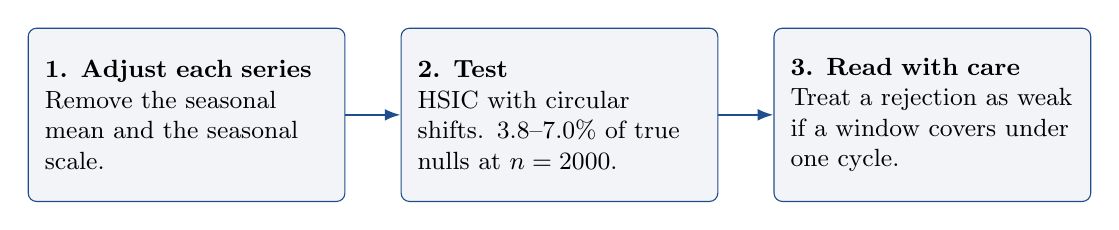
\begin{tikzpicture}[node distance=7mm, every node/.style={font=\small, align=left},
  box/.style={draw=ktblue, fill=ktblue!6, rounded corners=3pt, inner sep=6pt, text width=36mm, minimum height=22mm},
  arrow/.style={-{Latex[length=2mm]}, ktblue, thick}]
\node[box] (a) {\textbf{1. Adjust each series}\\Remove the seasonal mean and the seasonal scale.};
\node[box, right=of a] (b) {\textbf{2. Test}\\HSIC with circular shifts. 3.8--7.0\% of true nulls at $n=2000$.};
\node[box, right=of b] (c) {\textbf{3. Read with care}\\Treat a rejection as weak if a window covers under one cycle.};
\draw[arrow] (a) -- (b);
\draw[arrow] (b) -- (c);
\end{tikzpicture}
\end{center}
\begin{why}{EXP2, EXP3 and EXP4 together}
\begin{itemize}
\item The seasonal results give step 1, the size and power results give step 2, and the slow-drift result gives step 3.
\item The 3.8--7.0\% range excludes slow drift (10.1\%) and a shared fixed phase (28--34\%). In EXP7, inc1 with shifts gives 5.8\% and 6.5\% there (simulation only).
\item For split MMD the rules above did not hold size under memory. The block rule of hsplit2 is one partial fix. Its plug-in rule still has one rising cell.
\end{itemize}
\end{why}
\end{frame}

\begin{frame}
\frametitle{What was already known, and what is new}
\small
\begin{columns}[T]
\begin{column}{0.49\textwidth}
\begin{block}{Already known}\small
\begin{itemize}
\item The original tests assume i.i.d.\ data.
\item Time-series extensions assume mixing, which fGn with $H>1/2$ does not satisfy.
\item The line $H_X+H_Y=3/2$.
\item Oversized dCov subsampling (Betken, Dehling).
\item Seasonal-mean nonsense correlation (Yule, 1926).
\end{itemize}
\end{block}
\end{column}
\begin{column}{0.49\textwidth}
\begin{block}{New in this paper}\small
\begin{itemize}
\item How large the MMD and HSIC false alarms are, rule by rule, side by side.
\item Process features crossed with memory.
\item Seasonal scale as a kernel-specific failure.
\item Propositions 1 and 2.
\item A decision rule with power checked.
\end{itemize}
\end{block}
\end{column}
\end{columns}
\end{frame}

\begin{frame}
\frametitle{Closest prior work: Betken and Dehling, and where we differ}
\footnotesize
\renewcommand{\arraystretch}{1.0}
\vspace{-2mm}
\begin{tabular}{@{}>{\bfseries\raggedright}p{0.13\linewidth}>{\raggedright}p{0.39\linewidth}>{\raggedright\arraybackslash}p{0.42\linewidth}@{}}
\toprule
& Betken, Dehling (arXiv 2107.03041) & This paper \\
\midrule
Null, generator & Independent long-memory processes, fGn & The same, with process features added \\
Statistic & Lag-weighted dCov, Pearson as comparator & Gaussian-kernel HSIC, dCov, Pearson, split MMD \\
Critical value & Subsampling with offset $0.1n$ & Subsampling (same offset), wild, circular shifts \\
Theory & dCov limit if both $H<3/4$, or $H_X+H_Y>3/2$ with identity transforms & No new long-memory limit. Propositions 1 and 2 are on other objects \\
Memory, $n$ & $H=0.6, 0.7$ and $n\le1000$ & $H\le0.9$, unequal pairs, $n=2000$ (some to 8,000) \\
Features & Instantaneous transforms only & Tails, nonlinear dynamics, seasonality, crossed with $H$ \\
dCov size & 11.2--17.5\% at $H=0.7$ & 10.6\% at $H=0.7$, $n=2000$ \\
\bottomrule
\end{tabular}
\begin{why}{audit of arXiv v3}
They already have the null, the $H_X+H_Y=3/2$ line and oversized dCov subsampling, so we do not claim these. Our distinct part is the comparison of rules, the process features, split MMD and the two propositions.
\end{why}
\end{frame}

\begin{frame}
\frametitle{Five questions for Wednesday's call (1 of 2): the proofs}
\begin{block}{1. Can we prove the size of circular shifts?}\footnotesize
\begin{itemize}
\item \textbf{Where we stand.} An argument shows the shift rule's size is right asymptotically (inc1, and raw below 3/2), but it rests on an unreviewed preprint. Proved directly: inc1's statistic stays bounded at every $H<1$ at a fixed width. The finite-sample size is simulated only. Rates at $H=0.8$ are 5.7\%, 6.3\% and 8.3\% at $n=2000, 4000, 8000$. The last has 144 replications, with an interval of 4.8--14.0\%.
\item \textbf{Seasonal-mean sketch.} It lacks uniform convergence of $T_n(s)/n$ over offsets. It also lacks a treatment of the ties $h(d)=h(P/2-d)$, where lower-order long-memory terms decide.
\item \textbf{Ask.} Is a proof realistic, and for which case first? Or do we state the size as a measured result only?
\end{itemize}
\end{block}
\begin{block}{2. Do the two proofs hold up?}\footnotesize
\begin{itemize}
\item \textbf{Where we stand.} So far only a numerical script has checked them.
\item \textbf{Steps to read first.} The ergodic lemma with periodic weights, the HSIC limit $V_n\to h(D)$ under median bandwidths, and the invariance reduction behind the power bound.
\item \textbf{Citations to check.} Lehmann and Romano Theorem 6.2.1, Billingsley Theorem 2.8, and Cornfeld, Fomin and Sinai Chapter 14.
\item \textbf{Ask.} Will you read the proofs appendix before we submit?
\end{itemize}
\end{block}
\end{frame}

\begin{frame}
\frametitle{Five questions for Wednesday's call (2 of 2): the method and the venue}
\begin{block}{3. Is there a correction for slow drift?}\footnotesize
A seasonal scale with period $4n$ raises shifts to 10.1\% at $n=2000$, against 6.2\% at $n=500$, with no memory. In the stock windows, a smooth time-of-day adjustment leaves the within-window trend in place, in about 44\% of windows. We have no correction for raw HSIC. In EXP7, inc1 with shifts gives 5.8\% under slow drift and 6.5\% under a shared fixed season (simulation only). \textbf{Ask:} do we adopt inc1 as the correction, or state slow drift as a limit?
\end{block}
\begin{block}{4. Do we choose a data-driven bandwidth, or leave that out?}\footnotesize
EXP6 fixes the bandwidth at 0.5, 1, 2 and 4 times the median. Wider kernels gain power under a seasonal scale and lose it against the squared link, so no fixed multiple wins. Shifts hold size at all four. We did not study data-driven choice. \textbf{Ask:} is a new experiment worth the time, or is the stated limit enough?
\end{block}
\begin{block}{5. Which venue: a journal, or AISTATS?}\footnotesize
The draft has 25 pages. AISTATS would mean cutting to about 8, which would lose most of the evidence. The JFec special issue date of 1 September 2026 has passed. Betken and Dehling are the closest prior work, so any venue needs our distinction from them to be clear. \textbf{Ask:} which journal would you choose, or do you prefer the short route?
\end{block}
\end{frame}
\end{document}
